\chapter{Experiment on performance} % Main chapter title

\label{Chapter4} % Change X to a consecutive number; for referencing this chapter elsewhere, use \ref{ChapterX}



%----------------------------------------------------------------------------------------
%	SECTION 1
%----------------------------------------------------------------------------------------



The aim of this experiment is to evaluate the performance of the proposed collision avoidance method in comparison with the Holm's method by simulation.

\section{Design of simulation}
The results of two preceding experiments are applied to design a simulation. The time-dependent synced-rotational gain of 1.6 degrees per second and the curvature distance of 23cm at the distance of 4m (walking speed 0.5m/s x walking duration 8s) are employed to simulate the walking path of an agent. An agent walks at the speed of 0.5m/s and changes the direction where he/she walks for a randomly selected direction between 0 to 360 degrees every 4 seconds. The shoulder with of the agent is 46cm.



As for the physical area where agents walk, three patterns of Large, Medium, and Small are taken into consideration by referring to~\cite{PMID:18183898}. Large is an area of 21.375 x 15.075m, Medium is 28.5 x 20.1m and Small is 35.625 x 25.125m. An agent collides with a surrounding wall when the distance between the wall and the center of the agent is less than 23cm. The agent also collides with other agents when their center-to-center distance less than 46cm. When agents collide with others, the 2:1 turn~\cite{8798319} strategy is performed to resolve starvation. As for collision avoidance, the likelihood of colliding between agents is obtained by a collision prediction bar. A collision prediction bar is 4m long and its origin is placed at the center of each agent. Its direction comes from a linear regression line which is obtained from the path he/she walked past 8 seconds. A collision is predicted if two collision prediction bars overlap, and the given collision avoidance of the Holm's method and the proposed one is performed. The time-dependent rotational gain for the Holm's method and the time-dependent synced-rotational gain for the proposed method are set the same with 1.6deg/s and the duration is 8 seconds.

\newpage

Fig.~\ref{fig:Simulation_2} to Fig.~\ref{fig:Simulation_15} show some screenshots of the simulation. The colored dots indicate agents. The outer circle of the dot indicates their shoulder width of 46cm. The triangle on the dot indicates their facing direction.

\begin{figure}[H]\centering
	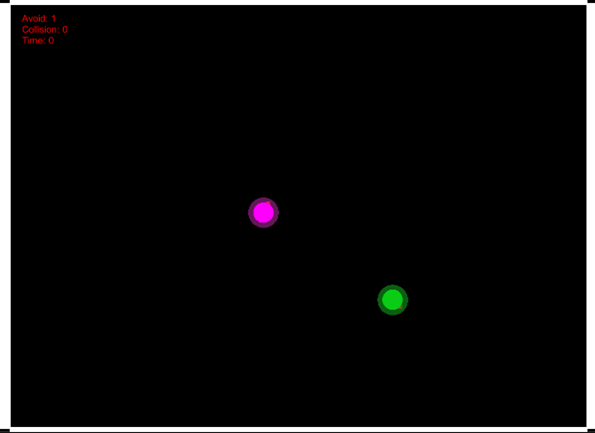
\includegraphics[width=0.9\textwidth]{Pictures/two users share real space.png}%imagine location
	\caption{Simulation for two users.}\label{fig:Simulation_2}%use name for ref.
	
\end{figure}


\begin{figure}[H]\centering
	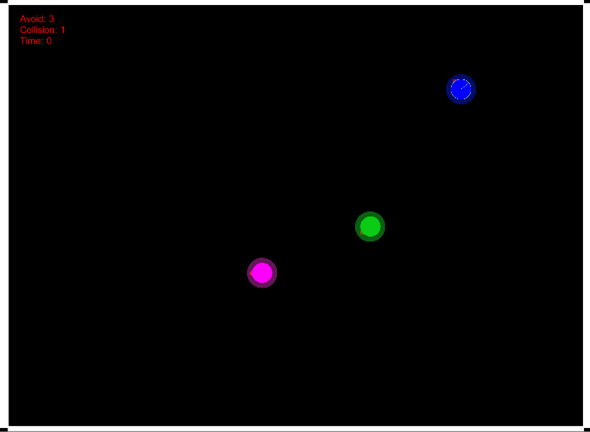
\includegraphics[width=0.9\textwidth]{Pictures/three users share real space.png}%imagine location
	\caption{Simulation for three users.}\label{fig:Simulation_3}%use name for ref.
	
\end{figure}


\begin{figure}[H]\centering
	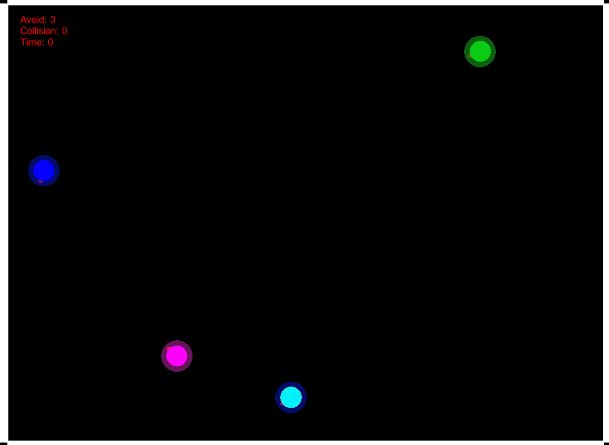
\includegraphics[width=0.9\textwidth]{Pictures/four users share real space.png}%imagine location
	\caption{Simulation for four users.}\label{fig:Simulation_4}%use name for ref.
	
\end{figure}


\begin{figure}[H]\centering
	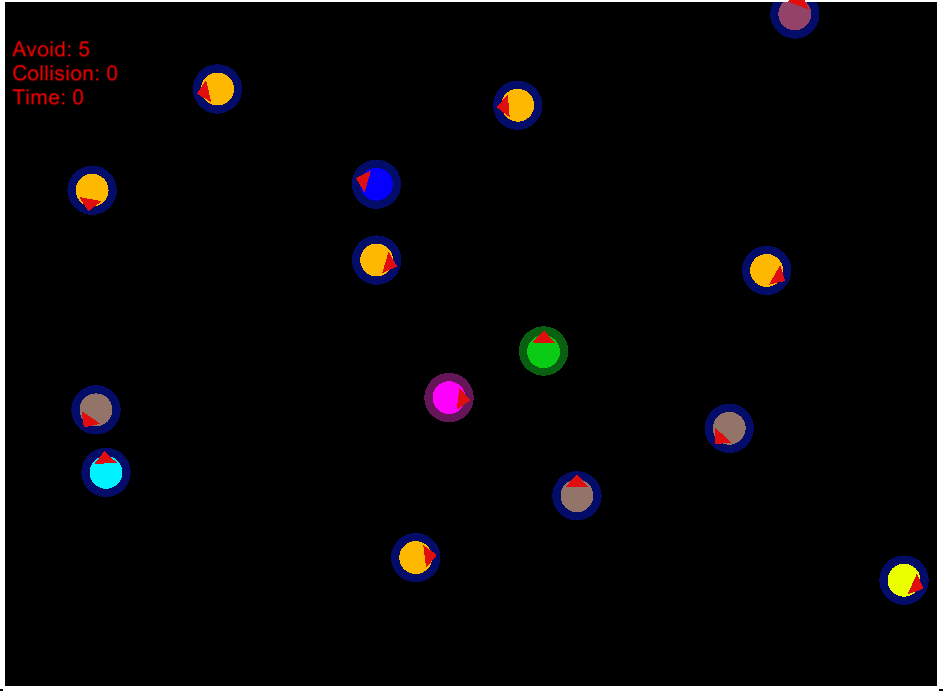
\includegraphics[width=0.9\textwidth]{Pictures/fifteen users share real space.png}%imagine location
	\caption{Simulation for fifteen users.}\label{fig:Simulation_15}%use name for ref.
	
\end{figure}

\newpage

\begin{table}[h!]\centering
	\caption{Data Collection.}
	\label{tab:Data CollectionEx3}%\scriptsize
		\scalebox{1.0}{
	\begin{tabular}{ |p{4cm}|p{3cm}|p{6cm}|}
	\hline
		Variable & Unit & Description \\\hline
		Count of avoidance & count &Number of occasions that a collision with other agents are successfully avoided.\\\hline
		Count of collision & count & Number of collisions with other agents that occur during the trial.\\\hline
		
		
	\end{tabular}
	}
\end{table} 

 A series of simulation is conducted under the following conditions. 14 patterns of agents (2$\sim$15) x 3 physical areas (Large, Medium and Small) x 10 trials x 2 methods = 840 trials in all. The data to be collected during each trial is summarised in Table.~\ref{tab:Data CollectionEx3}.

\newpage

\section{Results}
Fig.~\ref{fig:Area of 75 Percent} to Fig.~\ref{fig:Area of 125 Percent} show both the count of collisions and count of avoidance. The horizontal axis is the number of agents and the vertical one is the number of counts. The red line shows data from the Holm's method and the blue line shows data from the proposed method. The dash line is the count of collisions and the solid line is the count of avoidance. The three figures draw those lines at each different size of physical areas: Small, Medium and Large. From the results, it seems that as the area is larger, the counts of collisions and avoidance are reduced. Additionally, across all the number of agents for all the size of physical areas, the count of collisions for the proposed method is lower than the Holm's one.


Fig.~\ref{fig:Performance of the number of collisions} and Fig.~\ref{fig:Performance Averages} show a comparative improvement of the proposed method to the Holm's method. The horizontal axis is the number of agents and the vertical one is the percentage of the count of collisions from the proposed method for the one from the Holm's method at each different size of area (if the percentage is 100 percent, it means no improvement.) At Large area, an average of ratio is 80.22 percent. Fig.~\ref{fig:Performance Averages} shows the average and its standard deviation across all the number of agents at each different size of area.

Fig.~\ref{fig:Average of count of collisions} shows the average of counts of collisions at each different size of area for each method across all the number of agents. From the graph, there is a significant difference in the count of collisions between the Holm's method and proposed one for Medium and Large areas.  Fig.~\ref{fig:Average of count of collisions avoidance} shows the average of counts of avoidance at each different size of area for each method across all the number of agents. From the graph,  there is a significant difference in the count of  avoidance between the two methods for all the sizes of areas. The details of statistical evaluation are found in Appendix \ref{appendix:d} and Appendix \ref{appendix:e}.

Fig.~\ref{fig:Collision times average in all areas of our method} shows the average of counts of collisions at each the number of agents for each method across different sizes of areas. The count of collisions decreases after applying the proposed method over all the number of agents.  Fig.~\ref{fig:Avoidance times average in all areas of our method} indicates the average of counts of avoidance at each the number of agents for each method, the agents can avoid collisions better by 44.37\% in comparison with the Holm's method.

\newpage

\begin{figure}[H]\centering
	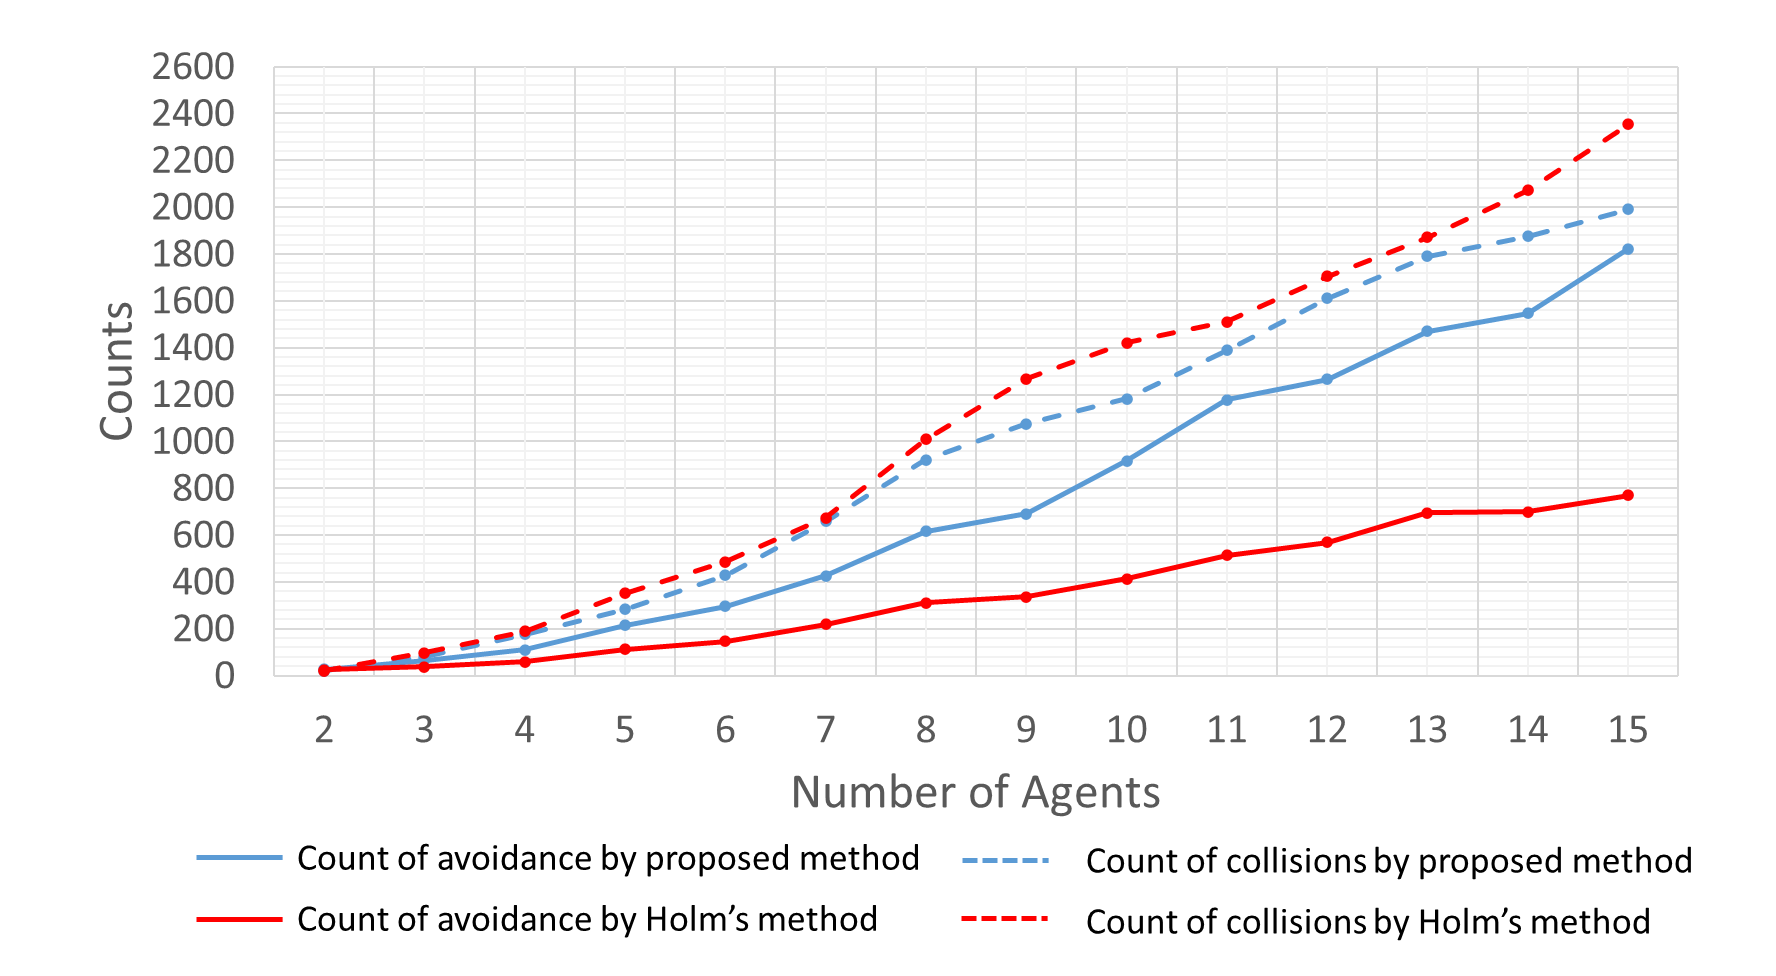
\includegraphics[width=1.0\textwidth]{Pictures/Area of 75 Percent.png}%imagine location
	\caption{Performance of collision avoidance for Small area.}\label{fig:Area of 75 Percent}%use name for ref.
	
\end{figure}

\begin{figure}[H]\centering
	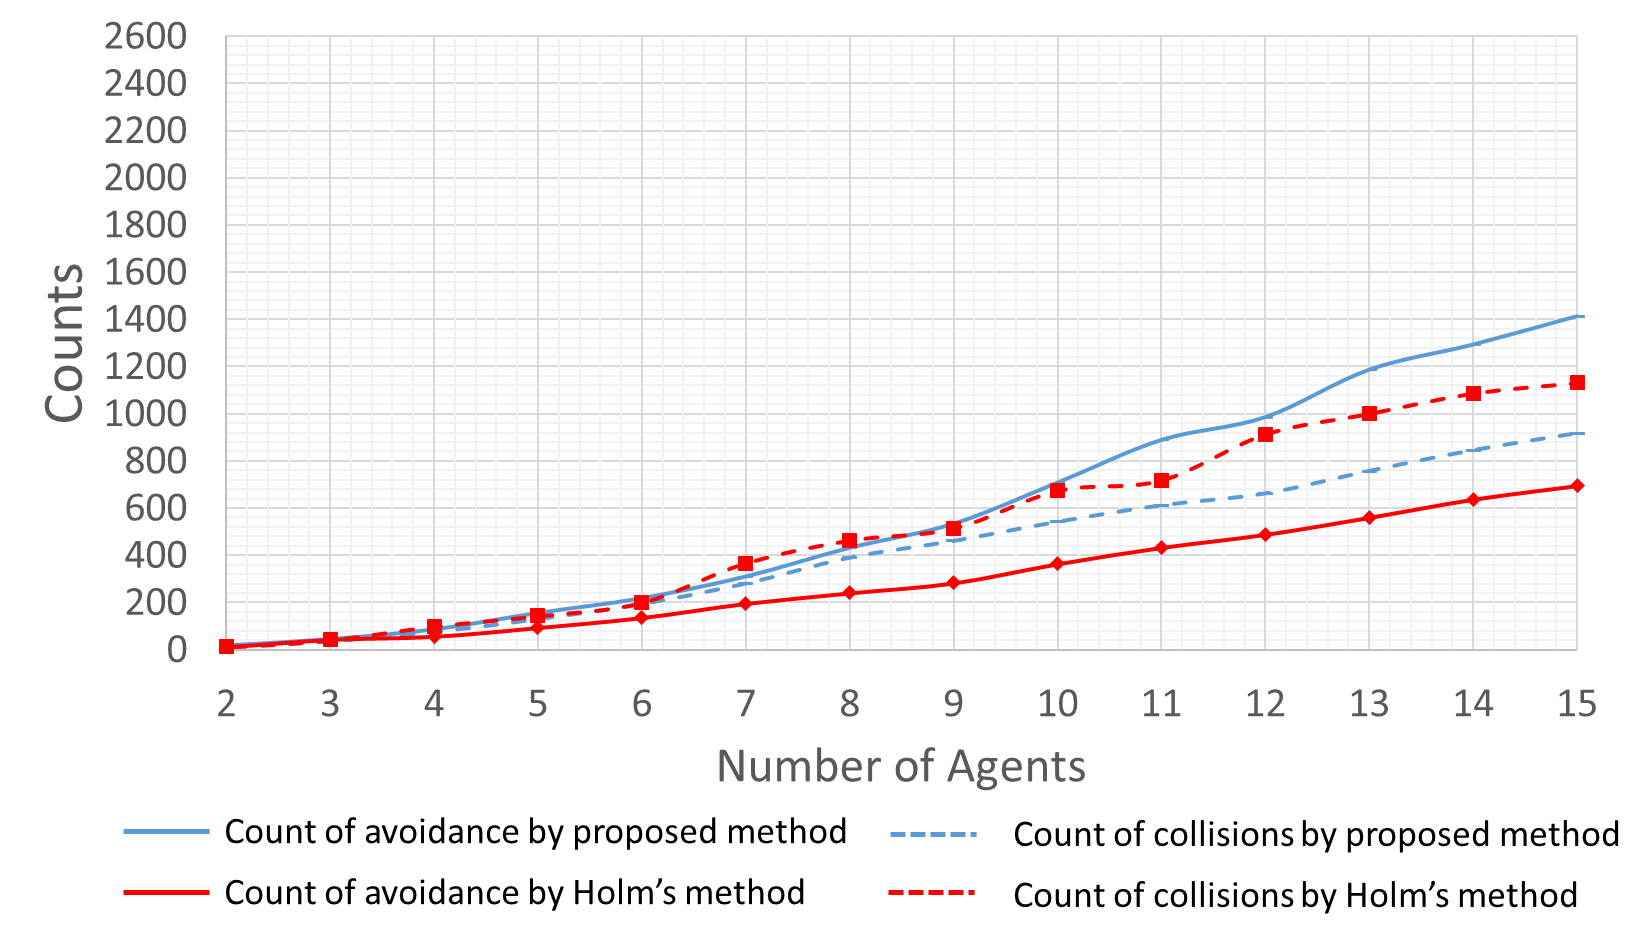
\includegraphics[width=1.0\textwidth]{Pictures/Area of 100 Percent.png}%imagine location
	\caption{Performance of collision avoidance for Medium area.}\label{fig:Area of 100 Percent}%use name for ref.
	
\end{figure}

\begin{figure}[H]\centering
	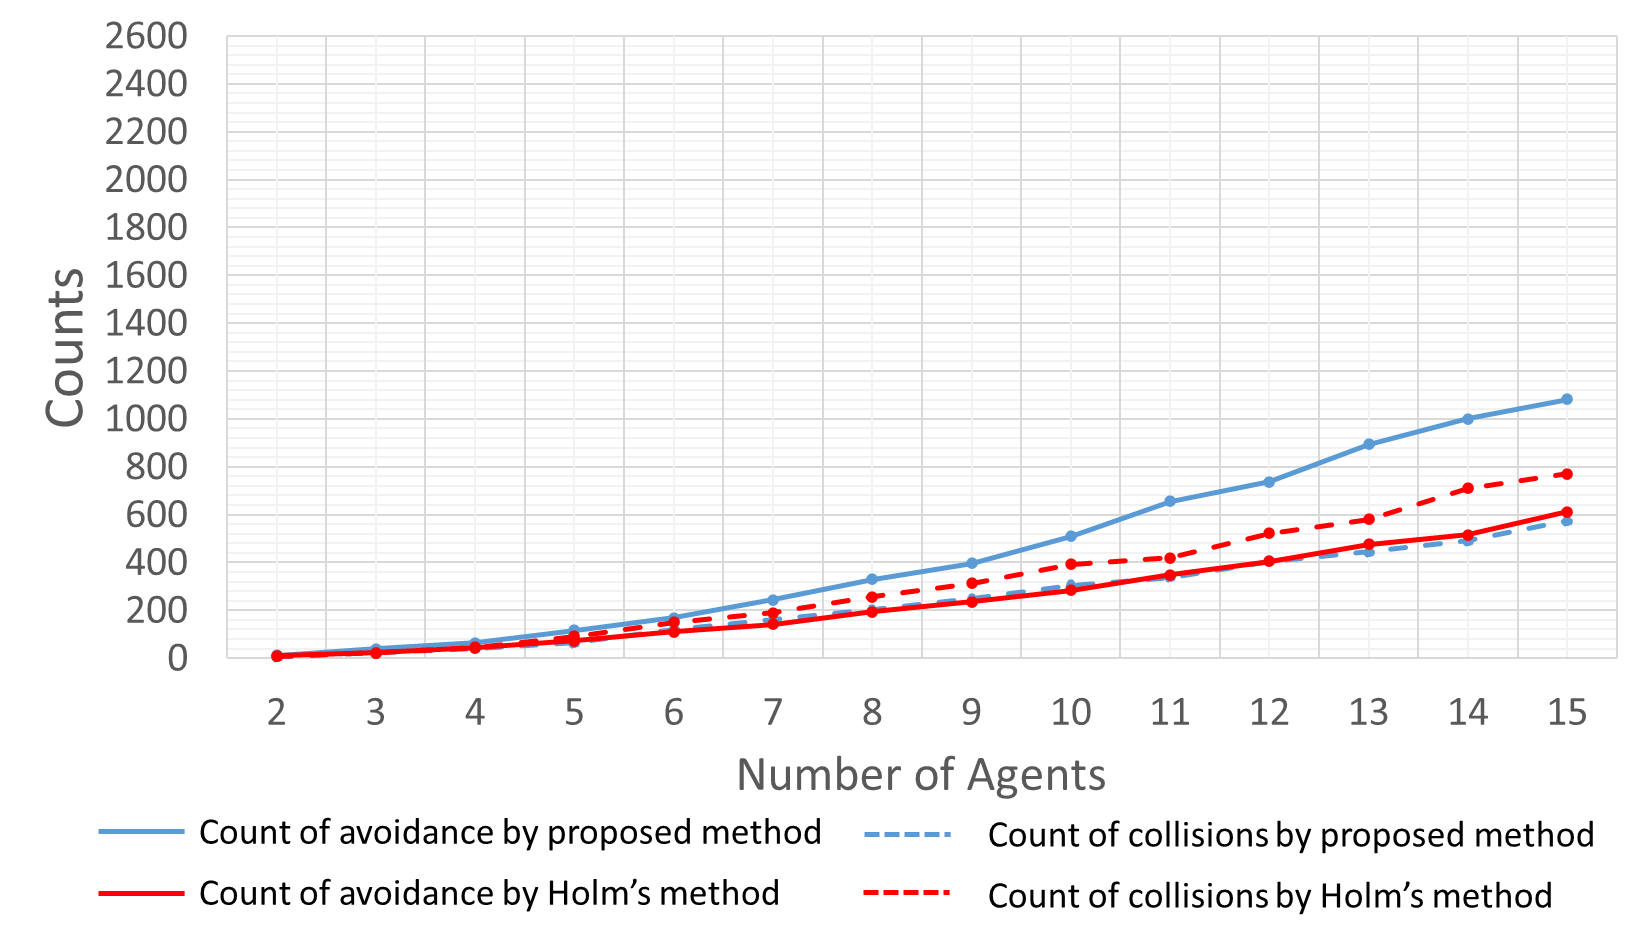
\includegraphics[width=1.0\textwidth]{Pictures/Area of 125 Percent.png}%imagine location
	\caption{Performance of collision avoidance for Large area.}\label{fig:Area of 125 Percent}%use name for ref.
	
\end{figure}
\newpage
\begin{figure}[H]\centering
	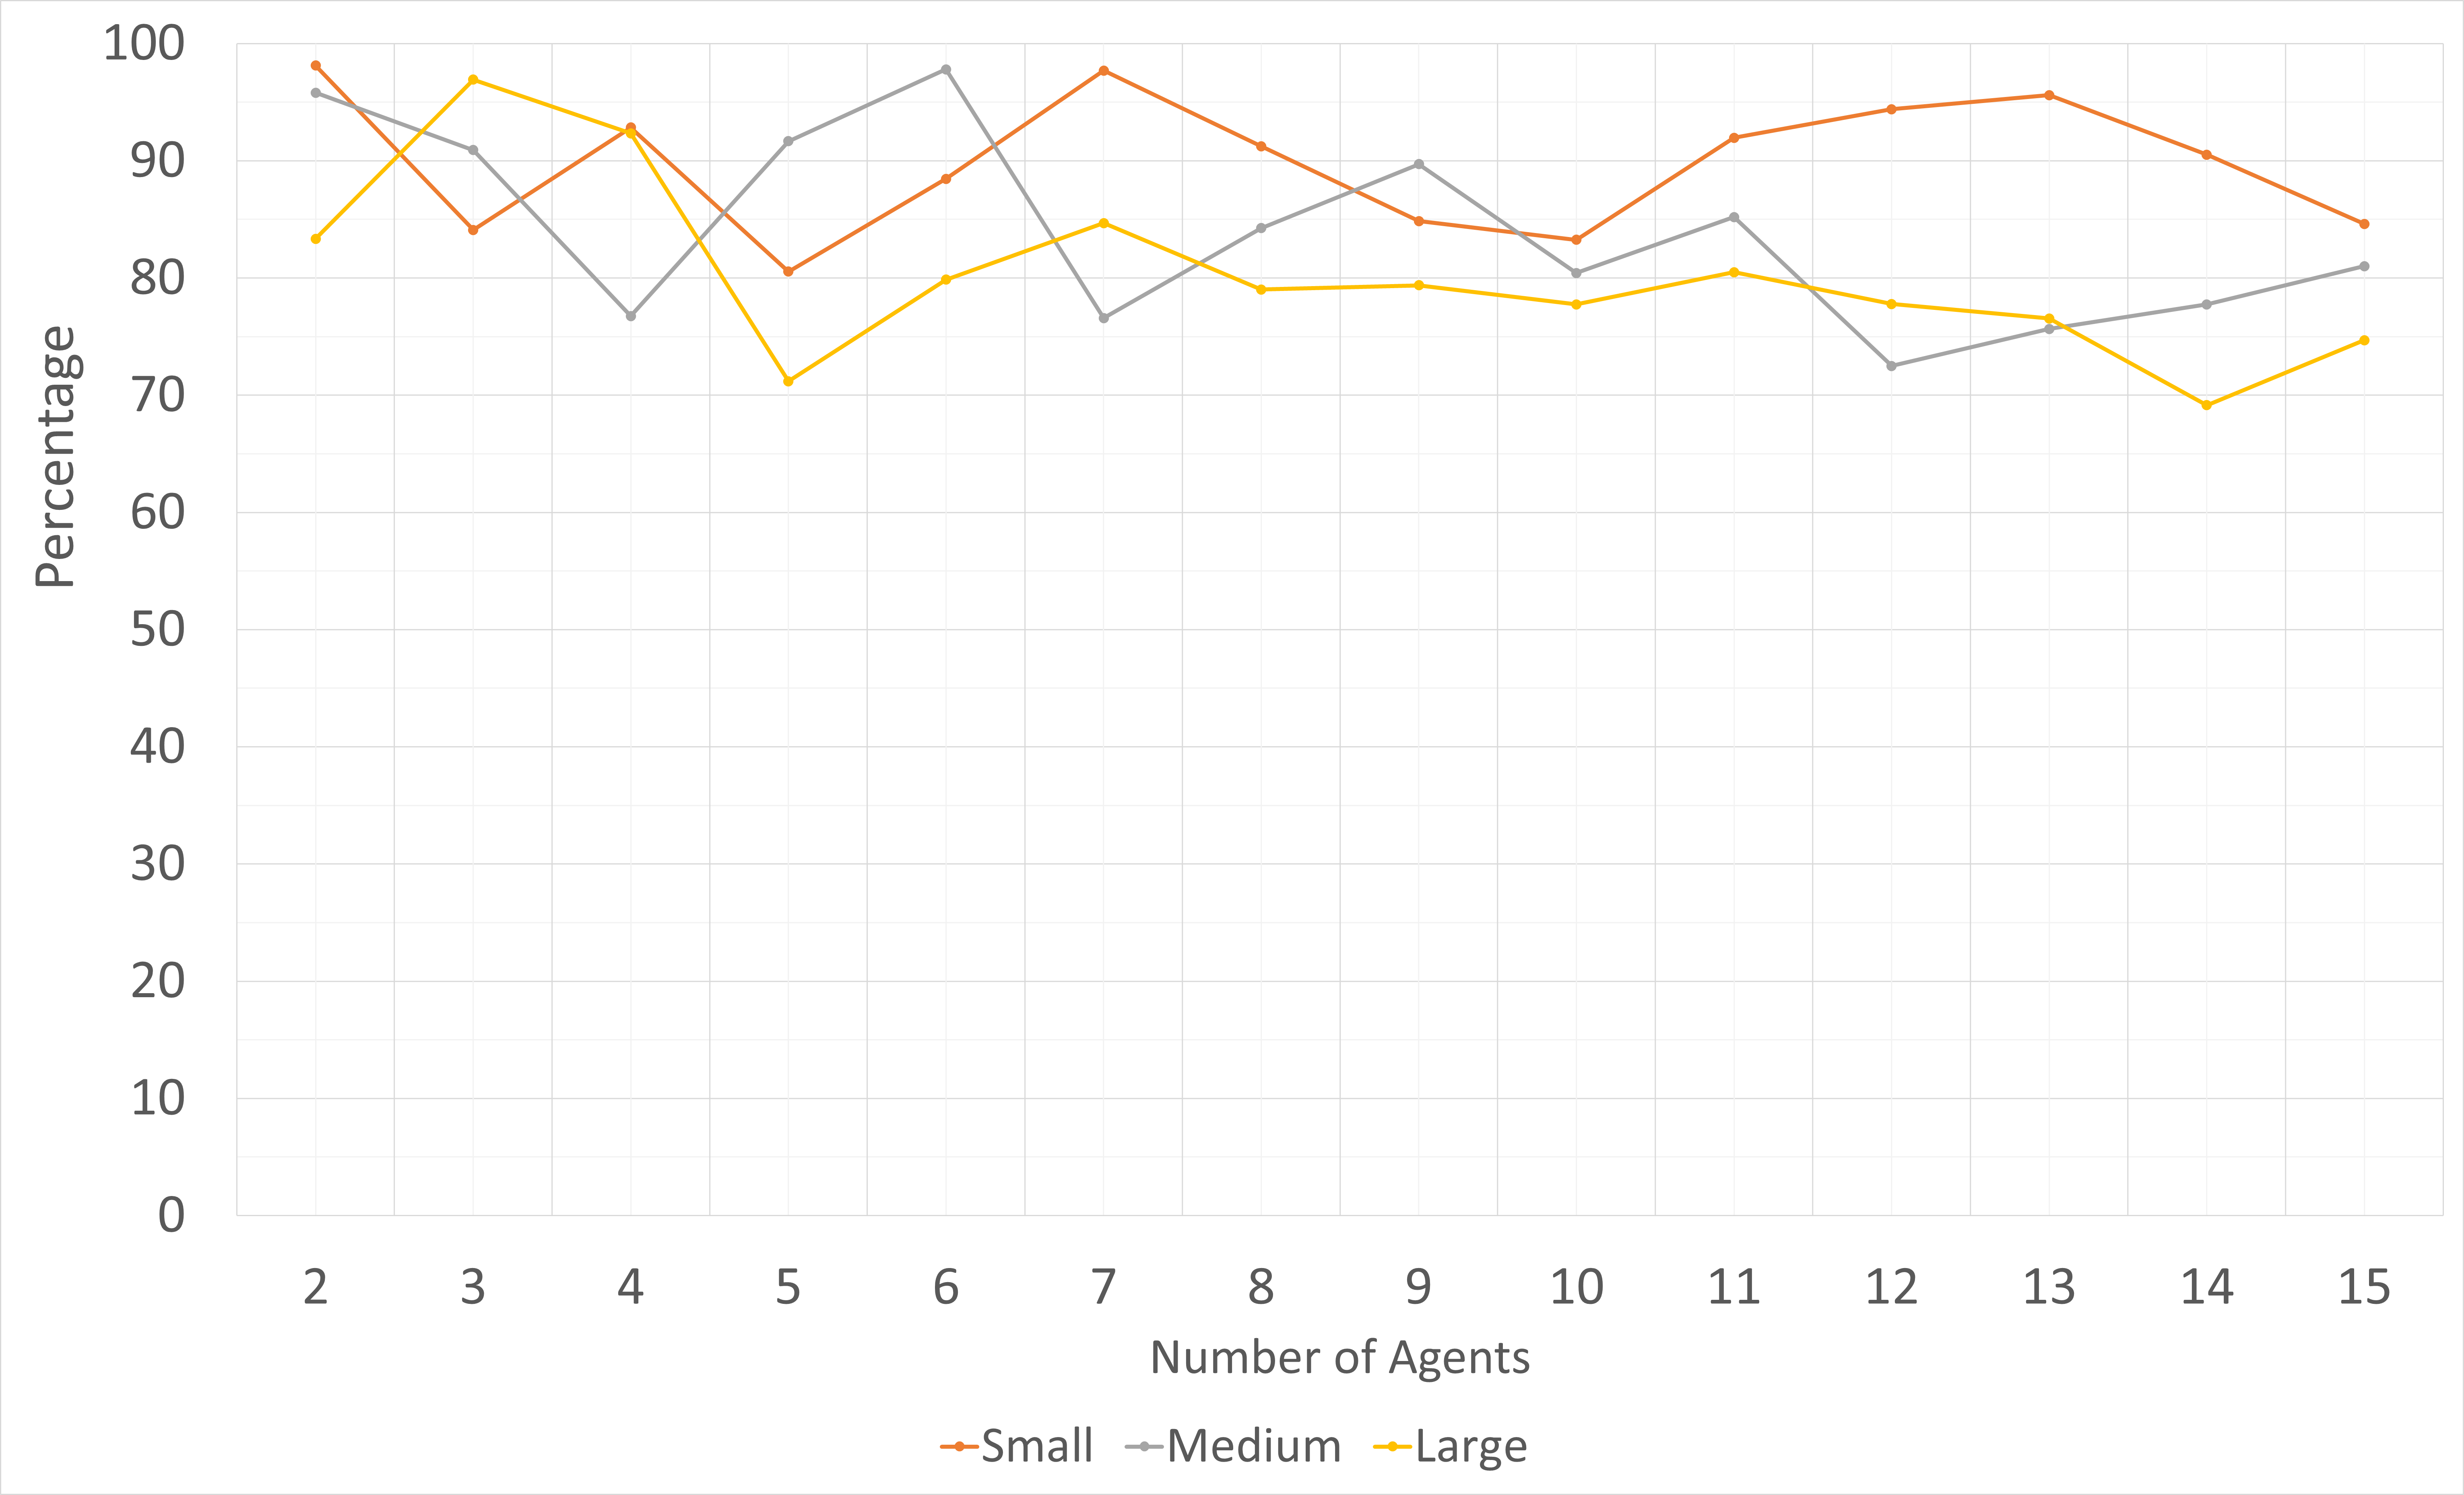
\includegraphics[width=1.0\textwidth]{Pictures/Performance of the number of collisions.png}%imagine location
	\caption{Improvement of the proposed method for the Holm's method in terms of the count of collisions.}\label{fig:Performance of the number of collisions}%use name for ref.
	
\end{figure}
\begin{figure}[H]\centering
	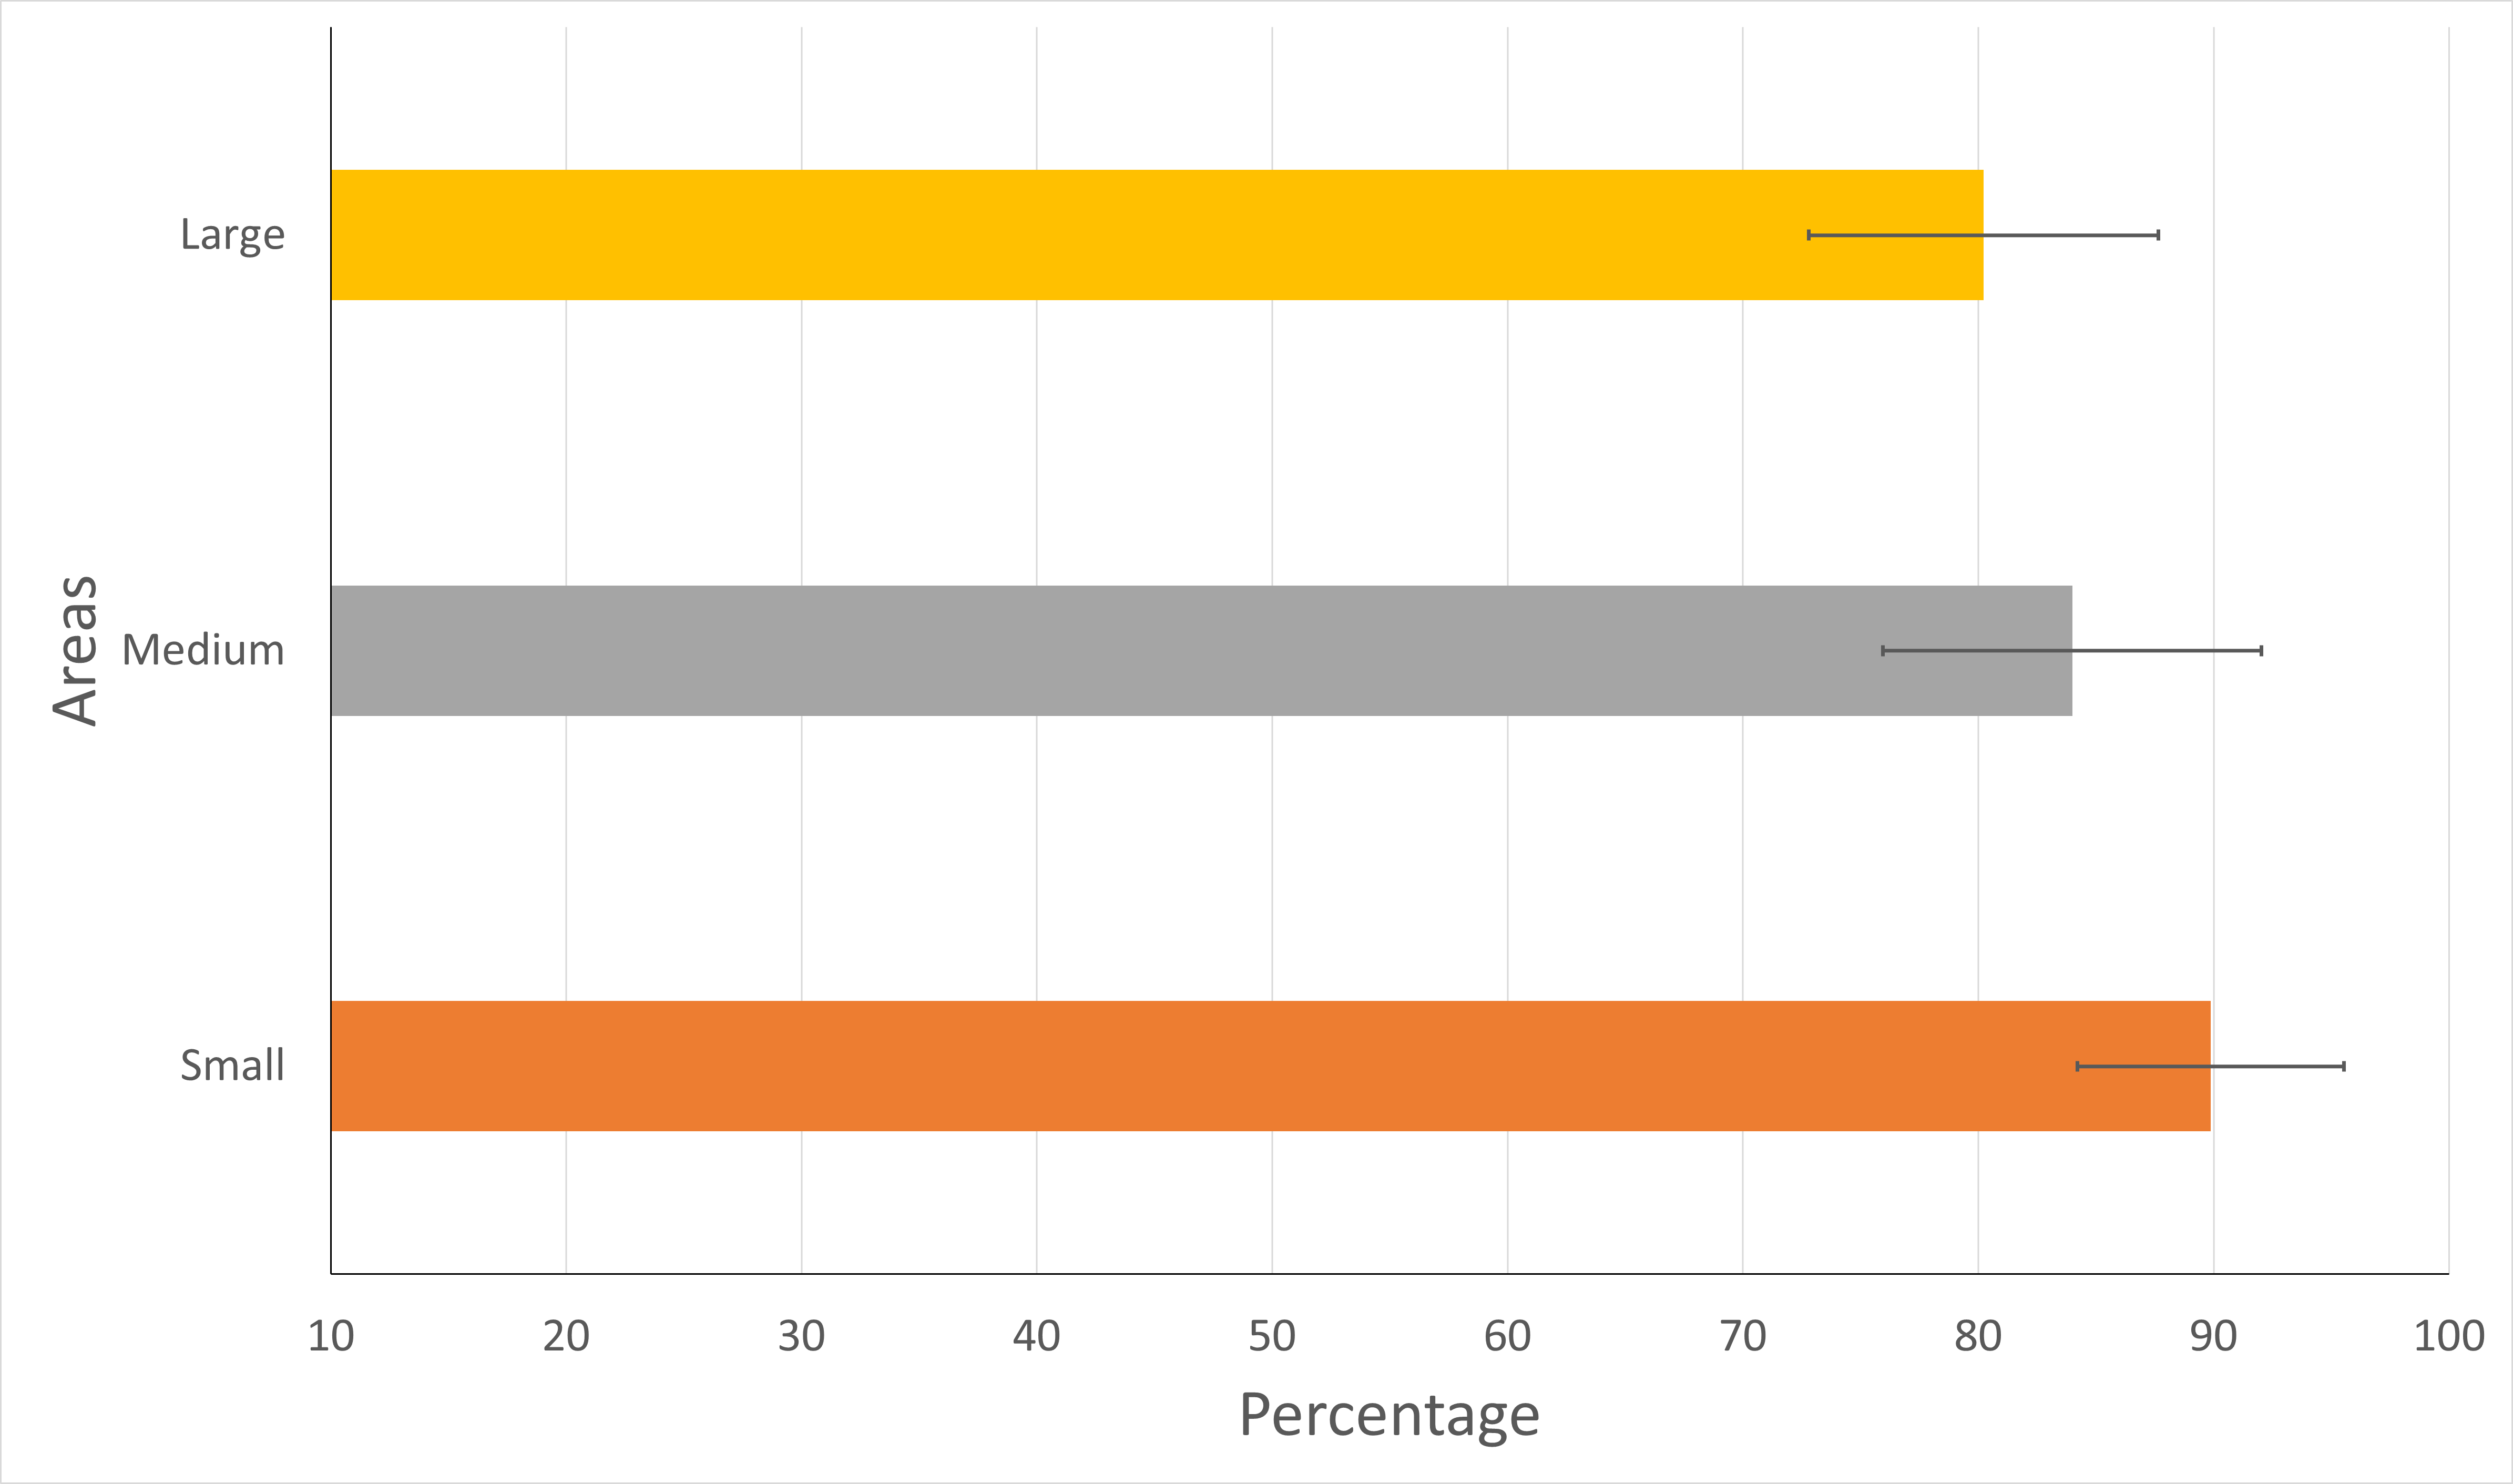
\includegraphics[width=1.0\textwidth]{Pictures/Performance Averages.png}%imagine location
	\caption{Average of the improvement.}\label{fig:Performance Averages}%use name for ref.
	
\end{figure}


\begin{figure}[H]\centering
	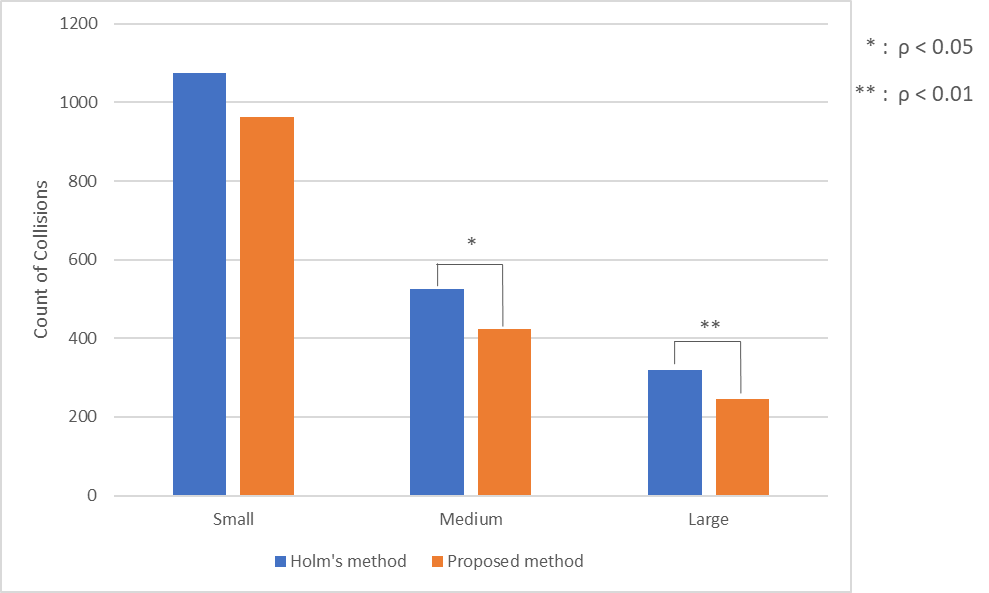
\includegraphics[width=1.0\textwidth]{Pictures/Average of count of collisions of each different of area.png}%imagine location
	\caption{Average of counts of collisions at each different size of area.}\label{fig:Average of count of collisions}%use name for ref.
	
\end{figure}
\begin{figure}[H]\centering
	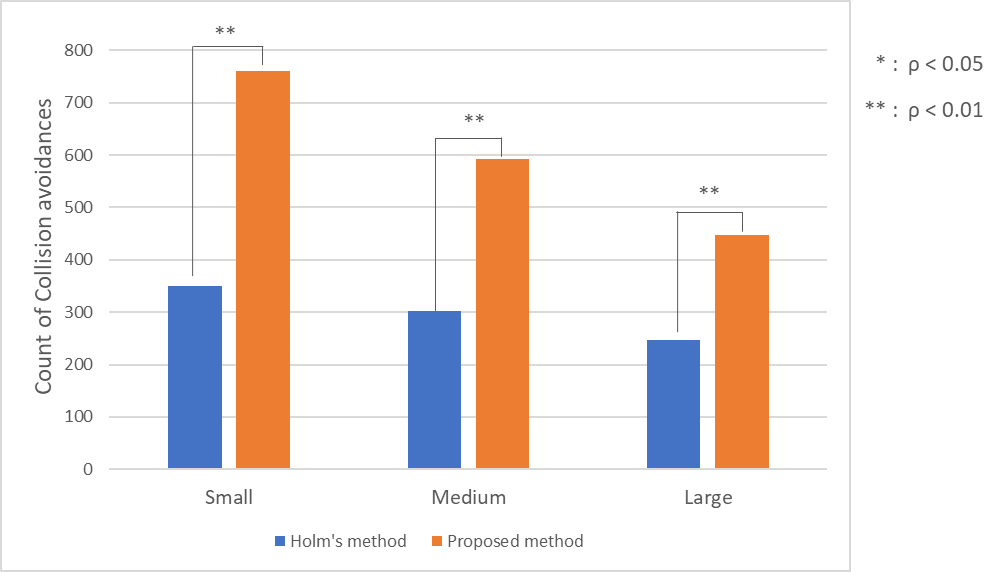
\includegraphics[width=1.0\textwidth]{Pictures/Average of count of avoidance of each different of area.png}%imagine location
	\caption{Average of counts of avoidance at each different size of area.}\label{fig:Average of count of collisions avoidance}%use name for ref.
	
\end{figure}
%\newpage




\begin{figure}[H]\centering
	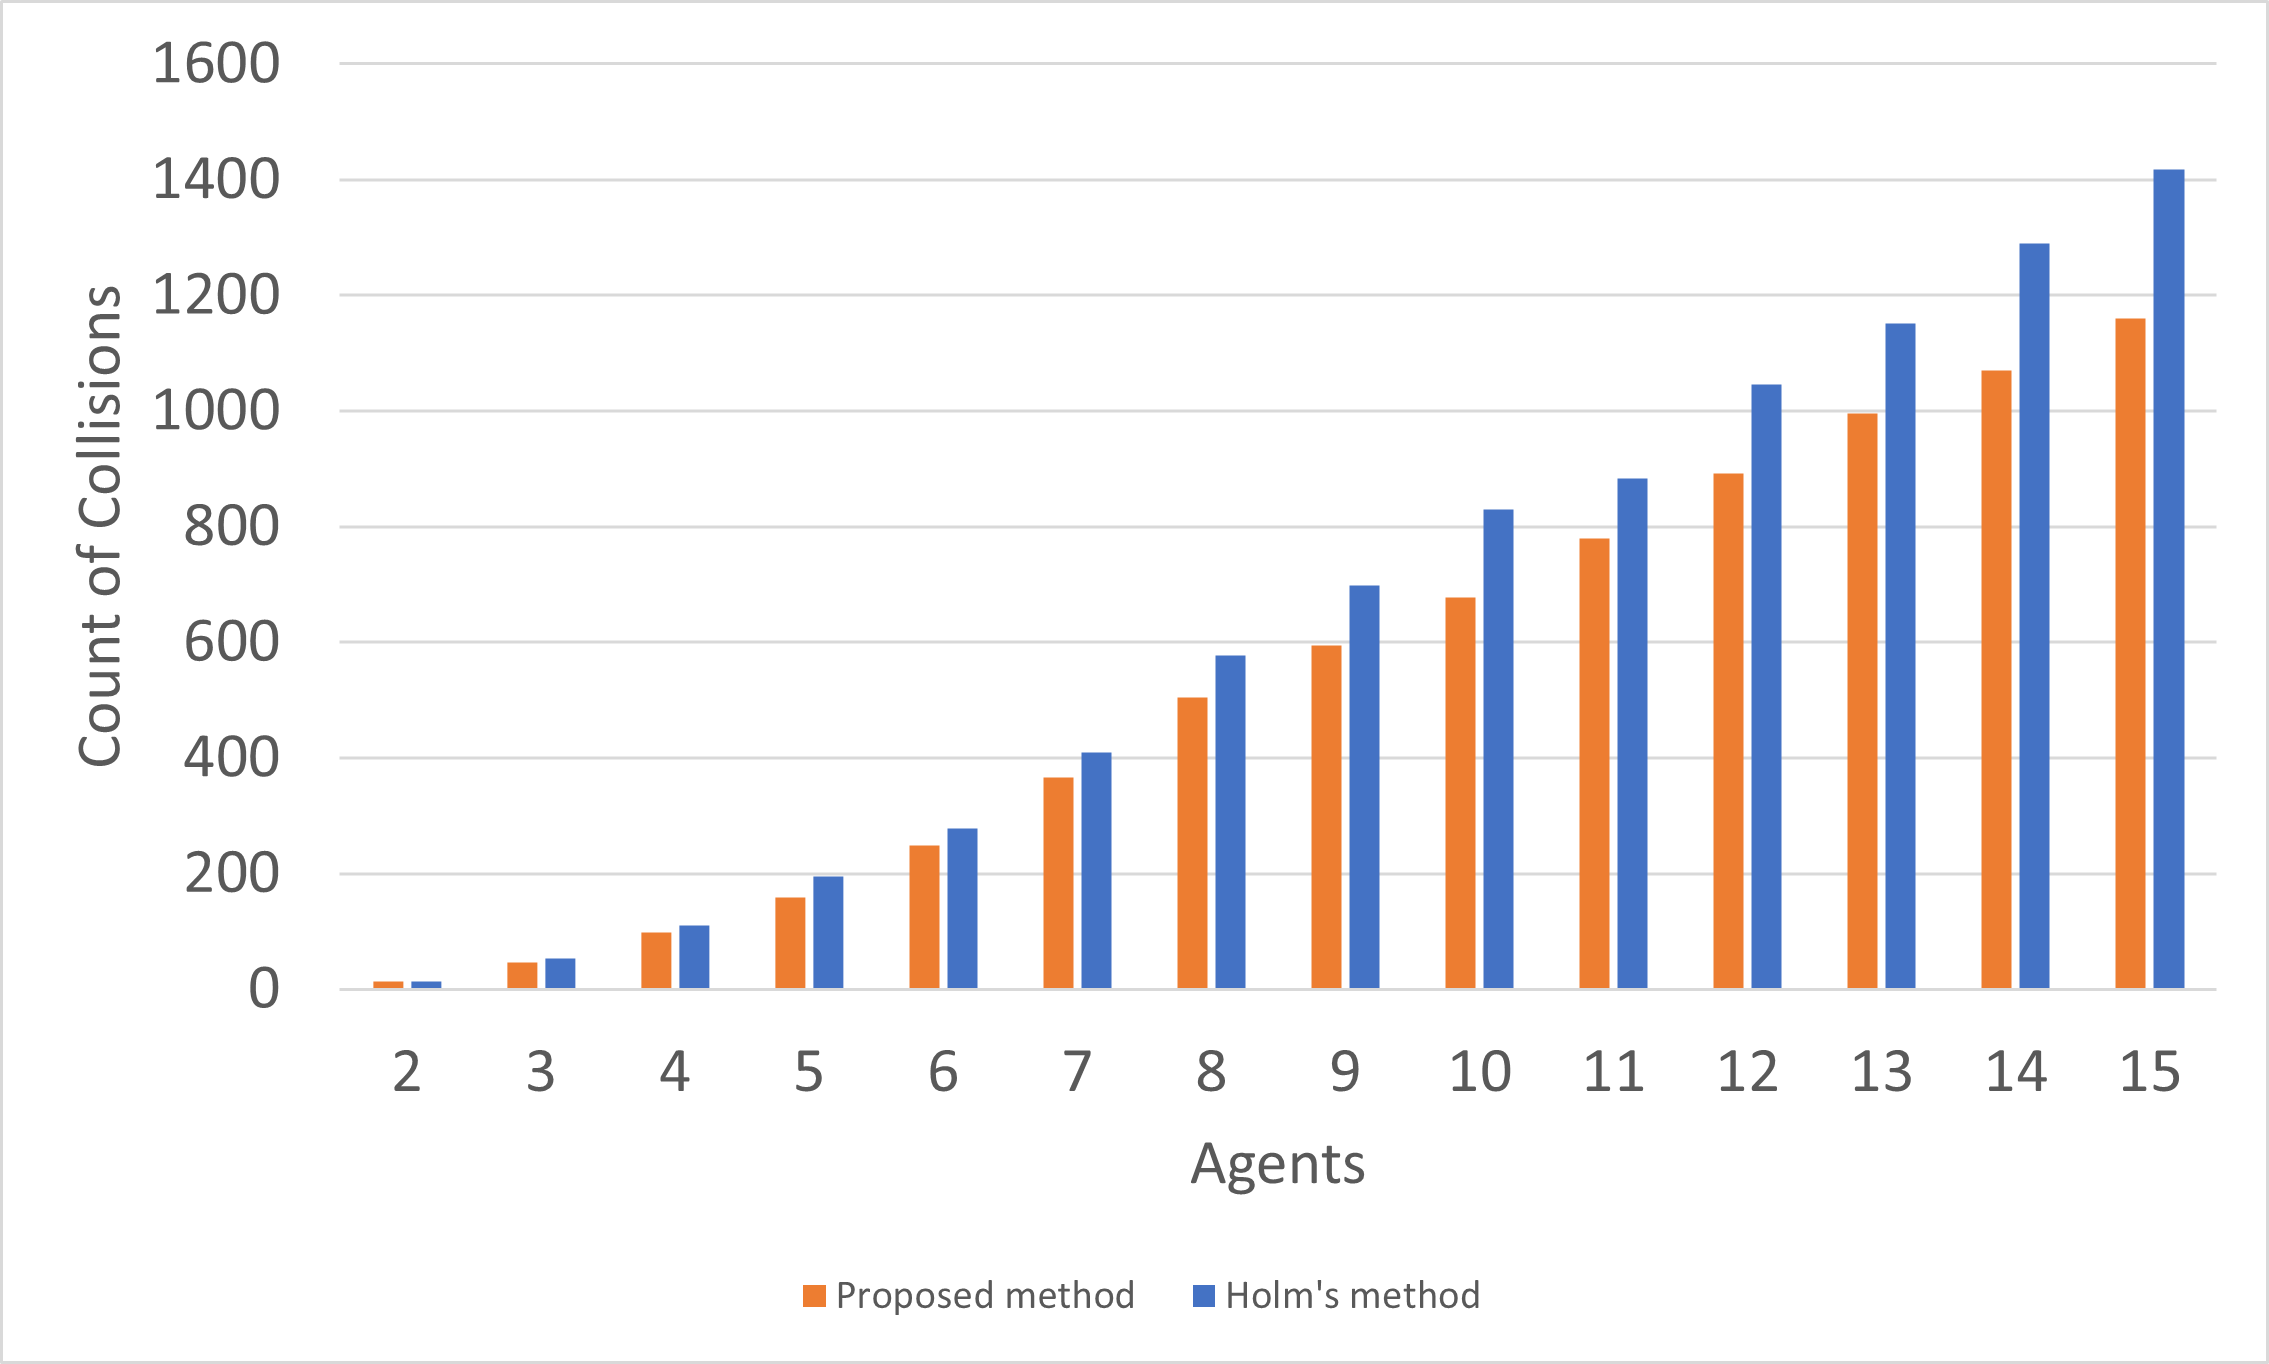
\includegraphics[width=1.0\textwidth]{Pictures/Average of count of collision of across all the number of user.png}%imagine location
	\caption{Average of counts of collisions at each the number of agents for each method.}\label{fig:Collision times average in all areas of our method}%use name for ref.
	
\end{figure}
\begin{figure}[H]\centering
	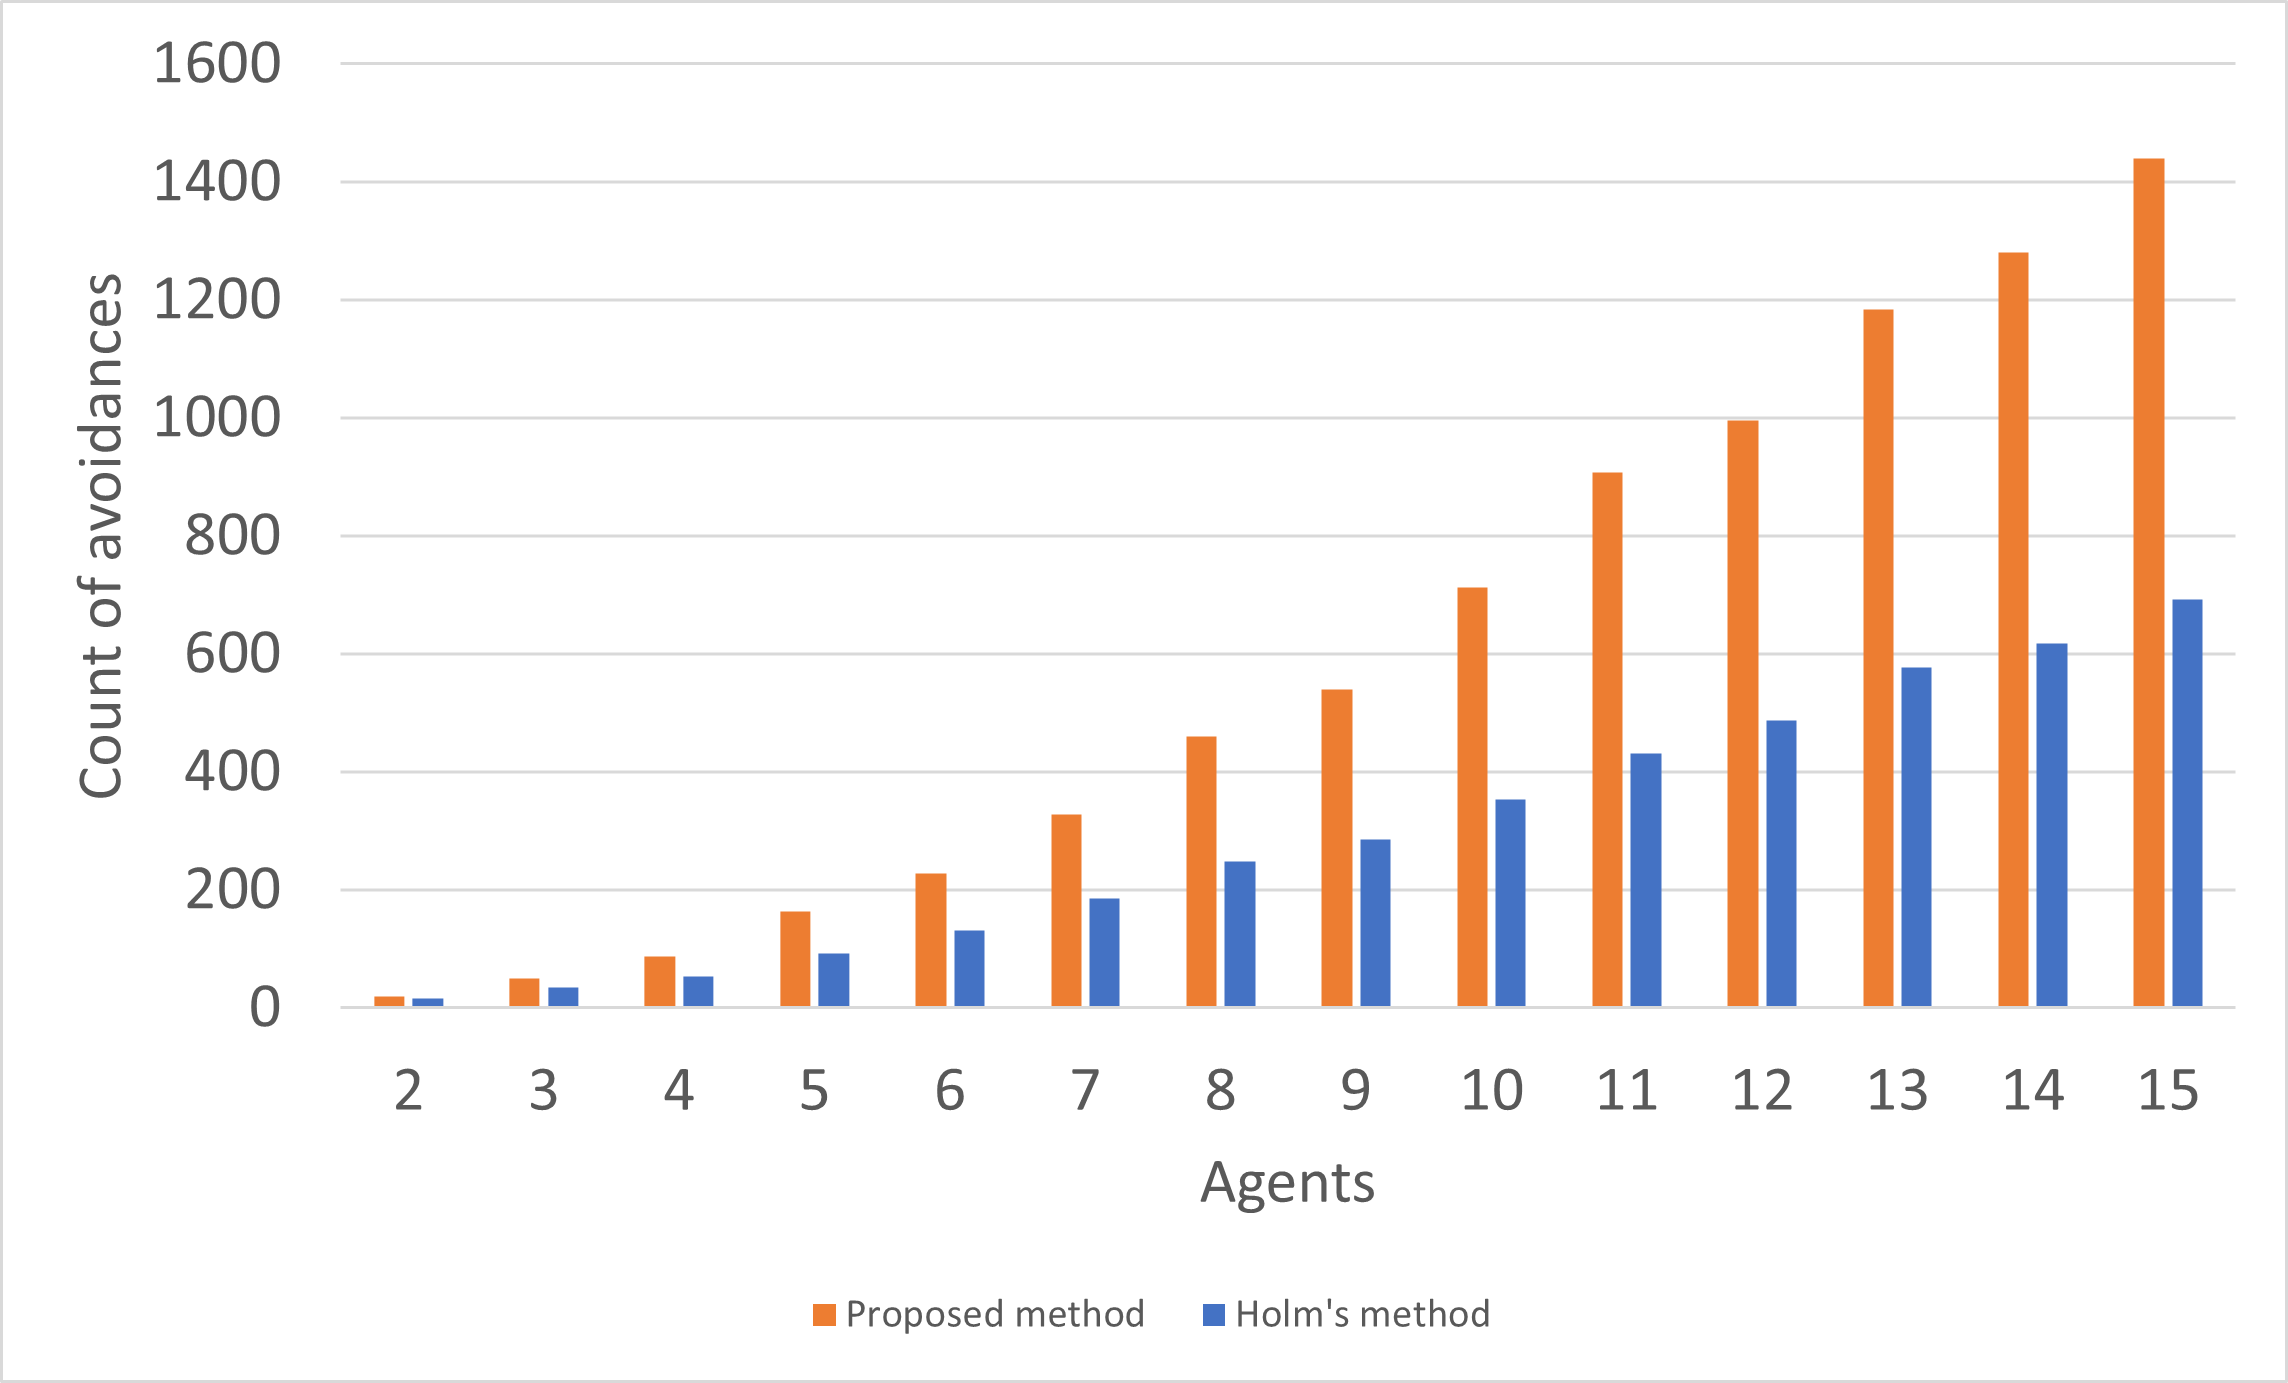
\includegraphics[width=1.0\textwidth]{Pictures/Average of count of collision avoidance of across all the number of user.png}%imagine location
	\caption{Average of counts of avoidance at each the number of agents for each method.}\label{fig:Avoidance times average in all areas of our method}%use name for ref.
	
\end{figure}




